\documentclass[11pt, addpoints, answers]{exam}

\usepackage{amsmath, amssymb}
\usepackage{xcolor}
\usepackage{tikz}

% headers, footers, titles
\newcommand{\CourseName}{CS101 Algorithms and Data Structures}
\newcommand{\HomeworkNO}{Homework 12}
\newcommand{\DueDate}{Due date: 23:59, December 21th, 2022}

\pagestyle{headandfoot}
\runningheadrule{}
\runningheader{\CourseName}{\HomeworkNO}{\DueDate}
\runningfooter{}{\thepage}{}

\title{
	\CourseName\\
	Fall 2022\\
	\HomeworkNO\\
}
\author{}
\date{\DueDate}

% formats of questions, choices, points, etc.
\qformat{\bf\thequestion. (\totalpoints\ points) \thequestiontitle\hfill}
\pointname{'}
\CorrectChoiceEmphasis{\bf\color{blue}}
\SolutionEmphasis{\color{blue}}

% We frequently use this font.
\newcommand{\ttt}{\texttt}
\newcommand{\bluett}[1]{\textcolor{blue}{\ttt{#1}}}

\begin{document}

\maketitle

\begin{enumerate}
	\item Please write your solutions in English.
	\item Submit your solutions to Gradescope.
	\item If you want to submit a handwritten version, scan it clearly.
	\item When submitting, match your solutions to the problems correctly.
	\item No late submission will be accepted.
	\item Violations to any of the above may result in zero credits.
	\item You are recommended to finish the algorithm design part of this homework with \LaTeX.
	\item Please check your Account Settings for Gradescope when submitting! Set your FULL name to your Chinese name and your 10-digit STUDENT ID correctly.
\end{enumerate}

\newpage

\renewcommand{\P}{\mathbf{\operatorname{P}}}
\newcommand{\NP}{\mathbf{\operatorname{NP}}}
\newcommand{\NPC}{\mathbf{\operatorname{NP-Complete}}}
\newcommand{\NPH}{\mathbf{\operatorname{NP-Hard}}}

\begin{questions}
	\titledquestion{Maximum Subarray Problem}

Given an array $A=\langle A_1, \dots, A_n\rangle$ of $n$ elements, please design a dynamic programming algorithm to find a contiguous subarray whose sum is maximum.

\vspace{0.05in}
{\large\textbf{Notes:}} \textcolor{red}{(MUST READ!)}

\begin{enumerate}
	\item Problems in this homework require you to design \textbf{dynamic programming} algorithms. When grading these problems, we will put more emphasis on how you define your subproblems, whether your Bellman equation is correct and correctness of your complexity analysis.
	\item \textbf{Define your subproblems clearly.} Your definition should include the variables you choose for each subproblem and a brief description of your subproblem in terms of the chosen variables.
	\item Your \textbf{Bellman equation} should be a recurrence relation whose \textbf{base case} is well-defined. You can briefly \textbf{explain each term in the equation} if necessary, which might improve the readability of your solution and help TAs grade it. 
	\item Analyze the \textbf{runtime complexity} of your algorithm in terms of $\Theta(\cdot)$ notation.
	\item You only need to calculate the optimal value in each problem of this homework, and you don't have to back-track to find the optimal solution.
\end{enumerate}

% utilities you might need for wrting Bellman equations
\newcommand{\maxi}[2]{\max\left\{#1,\ #2\right\}}	% usage: \maxi{a}{b}
\newcommand{\maxt}[3]{\max\begin{cases}#1\\#2\\#3\end{cases}}	% usage: \maxt{a}{b}{c}
\newcommand{\mini}[2]{\min\left\{#1,\ #2\right\}}	% usage: \mini{a}{b}
\newcommand{\mint}[3]{\min\begin{cases}#1\\#2\\#3\end{cases}}	% usage: \mint{a}{b}{c}
\newcommand{\case}[1]{\text{if}\ #1}	% usage: \case{$i > 1$}
\newcommand{\otherwise}{\text{otherwise}}	% usage: \otherwise

\vspace{0.05in}
\begin{parts}
	\part[0] Define your subproblem for this question.
	\begin{solution}
		$OPT(i)=$ the maximum sum of subarrays of $A$ ending with $A_i$.
	\end{solution}

	\part[0] Give your Bellman equation to solve the subproblems.
	\begin{solution}
		\[
			OPT(i)=
			\begin{cases}
				A_1                      & \case{i=1} \\
				\maxi{A_i}{A_i+OPT(i-1)} & \case{i>1}
			\end{cases}
		\]
		\paragraph{Explanation:} (NOT Required)
		\begin{itemize}
			\item The $1$st term in $\max$: only take $A_i$
			\item The $2$nd term in $\max$: take $A_i$ together with the best subarray ending with $A_{i-1}$
		\end{itemize}
	\end{solution}

	\part[0] What is the answer to this question in terms of the subproblems?
	\begin{solution}
		\[ \max_{i\in\{1, 2, \dots, n\}} OPT(i) \]
	\end{solution}

	\part[0] What is the runtime complexity of your algorithm?
	\begin{solution}
		$\Theta(n)$
	\end{solution}
\end{parts}
	\newpage

	\titledquestion{Multiple Choices}

Each question has \textbf{one or more} correct answer(s). Select all the correct answer(s). For each question, you will get 0 points if you select one or more wrong answers, but you will get 1 point if you select a non-empty subset of the correct answers.

Write your answers in the following table.

%%%%%%%%%%%%%%%%%%%%%%%%%%%%%%%%%%%%%%%%%%%%%%%%%%%%%%%%%%%%%%%%%%%%%%%%%%%
% Note: The `LaTeX' way to answer a multiple-choices question is to replace `\choice'
% with `\choice', as what you did in the previous questions. However, there are 
% still many students who would like to handwrite their homework. To make TA's work 
% easier, you have to fill your selected choices in the table below, no matter whether 
% you use LaTeX or not.
%%%%%%%%%%%%%%%%%%%%%%%%%%%%%%%%%%%%%%%%%%%%%%%%%%%%%%%%%%%%%%%%%%%%%%%%%%%

\begin{table}[htbp]
	\centering
	\begin{tabular}{|p{1.7cm}|p{1.7cm}|p{1.7cm}|p{1.7cm}|p{1.7cm}|p{1.7cm}|p{1.7cm}|p{1.7cm}|p{1.7cm}|}
		\hline
		(a) & (b) & (c) & (d) & (e) & (f) \\
		\hline
		%%%%%%%%%%%%%%%%%%%%%%%%%%%%%%%%%%%%%%%%%%%%%%%%%%%%%%%%%%
		% YOUR ANSWER HERE.
		    &     &     &     &     &     \\
		%%%%%%%%%%%%%%%%%%%%%%%%%%%%%%%%%%%%%%%%%%%%%%%%%%%%%%%%%%
		\hline
	\end{tabular}
\end{table}

\begin{parts}
    \part[2] A planar graph is a graph which can be embedded in a plane i.e. you can find a way to put all vertices on the plane where the edges will not intersect with each other. Which of the statement(s) is/are correct?
    \begin{choices}
        \choice $\forall n\leq 5, K_n$ is planar. $K_n$ means the complete graph with $n$ vertices.
        \choice $K_6$ is not planar.
        \choice DAGs are planar.
        \choice A tree is planar.
        \choice Bipartite graphs are planar.
    \end{choices}

    \part[2] Given a graph $G=(V,E)$, $w(e)$ indicates the weight of edge $e$. Which of the statement(s) is/are correct?
    \begin{choices}
        \choice Both Kruskal's and Prim's algorithms can correctly find the MST even when $\exists e, w(e)<0$.
        \choice Suppose $G$ is connected and $|E| = \omega(|V|)$, $G$ has a unique MST if and only if $\forall e,e'\in E, w(e) = w(e') \Leftrightarrow e = e'$ i.e. weights of edges are distinct.
        \choice Suppose $G' = (V,E)$ is the same graph as $G$ with different weight function $v(e)$. If they share a same MST $T$, then $T$ is also the MST of $G$ with weights $u(e) = w(e) + v(e)$.
        \choice If $G$ contains multi-edges i.e. $G$ is not simple, then Kruskal's algorithm will fail but Prim's won't fail when finding MST.
    \end{choices}

	\part[2] Given a graph $G=(V,E)$, which of the following is(are) correct? 
	\begin{choices}
		\choice If $G$ is a complete graph with $4$ vertices, then the number of spanning trees of $G$ is $16$.
		\choice After Kruskal's algorithm, we choose $m$ edges, then the number of connected components of $G$ is $|V|-m$.
		\choice If $G$ is stored in adjacency matrix, then the total time complexity of Kruskal's algorithm can reach $\Theta(|V|^2+|E|\log|E|)$.
        \choice Suppose $G$ is connected and $|V| = |E|$, the maximum number of spanning trees of $G$ can reach $\Theta(|V|)$.
	\end{choices}
    
    \part[2] Let $G$ be a weighted undirected graph with positive weights where edge $e$ has weight $w_e\in \mathbb{R}^+$ for all $e \in E$. A new graph $G'$, which is a copy of $G$, and the weight of each edge $e$ in $G'$ is transformed using a function $f(w_e)$. Which of the following statements is/are true?

    \begin{choices} 
        \choice If $f(w_e) = w_e^2$, then any MST in $G$ is also an MST in $G'$.
        \choice If $f(w_e) = 2^{w_e}$, then any MST in $G$ is also an MST in $G'$.
        \choice If $f(w_e) = \frac1 {w_e}$, then any MST in $G$ is also an MST in $G'$.
        \choice If $f(w_e) = \log (w_e)$, then any MST in $G$ is also an MST in $G'$.
    \end{choices}

	\part[2] What is the number of spanning trees of following graph?

    \begin{center}
    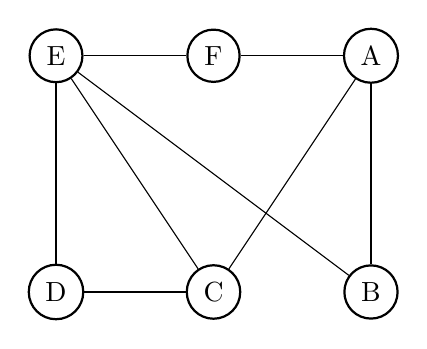
\begin{tikzpicture}
        \begin{scope}[every node/.style = {circle, thick, draw}]
            \node (A) at (2,0) {A};
            \node (B) at (2, -3) {B};
            \node (C) at (0, -3) {C};
            \node (D) at (-2, -3) {D};
            \node (E) at (-2, 0) {E};
            \node (F) at (0,0) {F};
        \end{scope}
        \begin{scope}
            \path[-] (E) edge (D);
            \path[-] (E) edge (C);
            \path[-] (E) edge (B);
            \path[-] (C) edge (D);
            \path[-] (B) edge (A);
            \path[-] (A) edge (C);
            \path[-] (A) edge (F);
            \path[-] (E) edge (F);
        \end{scope}
    \end{tikzpicture}
    \end{center}
	\begin{choices}
		\choice 32
		\choice 34
		\choice 36
		\choice 38
	\end{choices}

        \part[2] Which of the following statements are true for MST(Minimum Spanning Tree)?
        \begin{choices}
            \choice Suppose $G$ has multiple MSTs. For each minimum spanning tree $T$ of a graph $G$, there is a way to sort the edges of $G$ in Kruskal’s algorithm so that the algorithm returns $T$.
            \choice Prim's algorithm is a divide-and-conquer algorithm because it divides the graph into $S$ and $V-S$ then solve.
            \choice If we use binary heap to optimize Prim's algorithm when choosing the next edge, it will always have a better time complexity than the original algorithm on any graph.
            \choice If we add a new edge $e = (u,v)$ into a graph $G=(V,E)$ with unique MST to get a new graph $G' = (V,E\cup\{e\})$. There is at most $1$ edge difference between the MST of $G$ and $G'$.
        \end{choices}

\end{parts}

	\newpage

	\titledquestion{PARTITION is $\NPC$}

Given an array \(A=[a_1,a_2,...,a_n]\) of non-negative integers, consider the following problems:

\textbf{1.Partition}: Determine whether there is a subset $P\subseteq[n] ([n]=\{1,2,...,n\})$ such that $\sum_{i\in P} a_i = \sum_{j\in[n]\backslash P} a_j $.\\
For example, given $A=[2,4,6,8]$, then $P=\{1, 4\}$ is a partition of $A$ since $a_1+a_4=a_2+a_3=10$.

\textbf{2.Subset Sum}: Given some integer $K$, determine whether there is a subset $P \subseteq [n]$ such that $\sum_{i\in P}a_i = K$.\\
For example, given $A=[1, 3, 5, 7]$ and $K=6$ , then $P=\{1, 3\}$ gives a subset sum of $a_1+a_3=6$.

Suppose we have proven that Subset Sum problem is in NP-complete, prove that Partition problem is also in NP-complete.

\begin{parts}
  \part[2] Prove that the partition problem is in NP.
  \begin{solution}
    % \vspace{5ex}
    \\for any given partition $P$\\
    we can calculate $s_1 = \sum_{i\in P}a_i$, and $s_2 = \sum_{i\in [n]\backslash P}a_i$\\
    both $s_1,s_2$ can be compute in polynomial time.\\
    we just need to check whether $s_1=s_2$ or not.\\
    so the partition problem is in NP\\
  \end{solution}
  \part[7] Find a polynomial time reduction from subset sum problem to parittion problem, and prove its correctness.
  \begin{solution}
    % \vspace{50ex}
    \\let $M=\sum_{i\in [n]}a_i$,\\
    and let $N$ be a number that is big enough, such as take $N>10M$,\\
    we can generate a new array $A'=[a_1,a_2,\cdots,a_n,N-k,N+k-M]$\\
    and below we all talk about the new array $A'$.\\

    $\Rightarrow:$ if the Subset Sum problem $(A,k)$ is a yes-instance,\\
    then there exist a partition $P\subseteq [n]$ s.t. $\sum_{i\in P}a_i=k$\\
    let $P'=P\cup \{n+1\}$,\\
    so $\sum_{i\in P'}a_i=k+(N-k)=N$\\
    and since $\sum_{i\in [n+2]\backslash P'}a_i=(M+(N-k)+(N+k-M))-N=N$\\
    which means that $\sum_{i\in P'} a_i = \sum_{j\in[n+2]\backslash P'} a_j $\\
    so the partition problem is yes-instance.\\

    $\Leftarrow:$ if the partition problem is yes-instance\\
    then there must exist a partition $P,s.t. \sum_{i\in P} a_i = \sum_{j\in[n+2]\backslash P} a_j $
    and since we took $N$ as a very big number that $N>10M$,\\
    so $a_{n+1}+a_{n+2}=(N-k)+(N+k-M)=2N-M>M$,\\
    so we can make sure that $a_{n+1}=N-k,a_{n+2}=N+k-M$ is impossible to be in the same partition.\\
    Without loss of generality, we suppose that $(n+1)\in P$, then $(n+2)\in [n+2]\backslash P$\\
    and since for the partition problem, each sum of the partition is half of the sum of the whole array,
    i.e. the value is $\frac{\sum_{i\in [n+2]}a_i}{2}=\frac{M+(N-k)+(N+k-M)}{2}=N$,\\
    so $\sum_{i\in P\backslash \{n+1\}}a_i=N-(N-k)=k$,\\
    so $(A,k)$ is a yes-instance, i.e. the Subset Sum problem is a yes-instance.\\
    and all operations we have done are in polynomial time.\\

    so above all, the subset sum problem can be reducted to partition problem in polynomial time.\\
		i.e. subset sum problem$\leq _p$ partition problem\\


  \end{solution}
  \part[1] Conclusion:
  \begin{solution}
    % \vspace{5ex}
    \\the partition problem is in $NP$\\
    the subset sum problem can be reducted to the partition problem in polynomial time\\\\
    let $A$ be the partition problem, $B$ be the subset sum problem,\\
    since $B\in NP-complete, B\leq _PA, A\in NP$\\
    so $A\in NP-complete$.\\\\
    so the partition problem is also in $NP-Complete$.\\

  \end{solution}
\end{parts}
\color{black}

	\newpage

	\newcommand{\HC}{\operatorname{HALF-CLIQUE}}
\newcommand{\CLQ}[1]{\operatorname{{#1}-CLIQUE}}
\titledquestion{$\HC \in \NPC$}

In an undirected graph $G=(V,E)$, a subset of the vertices $S\subseteq V$ is said to be a \textbf{clique}
if for all pairs of vertices in $S$ are connected or formally $\forall (u,v)\in S\times S (u\neq v\to \{u,v\}\in E)$.\\
Note that a subset of zero or one vertex is also considered as a clique.\\

The $\CLQ{k}$ problem is a classic $\NPC$ problem stated as follows:\\
Given $(k,G)$ where $k$ is a non-negative integer and $G$ is an undirected graph,
determine if $G$ contains a clique of at least $k$ vertices.\\

Now let's consider the $\HC$ problem which is defined as follows:\\
Given an undirected graph $G=(V,E)$, determine if $G$ contains a clique of $\lfloor V/2 \rfloor$ vertices.\\
Show that $\HC$ is a $\NPC$ problem.\\

\textbf{Hint}: reduce from $\CLQ{k}$, consider the cases where $k=|V|/2$, $k<|V|/2$ and $k>|V|/2$.


\begin{parts}
	\part[2]{$\HC\in \NP$}
	\begin{solution}
		% \vspace{5ex}
		\\for a given vertex set $S \subseteq V$,\\
		when can check whether $|S|=\lfloor\frac{|V|}{2}\rfloor$ in polynomial time.\\
		If so, we can check whether $\forall (u,v)\in S\times S (u\neq v\to \{u,v\}\in E)$ in polynomial time.\\
		If all these two checks are satisfied, then the half-clique is hold, we can check it in polynomial time.\\
		so above all, $\HC\in \NP$\\
	\end{solution}
	\part[7]{Polynomial time reduction: construction and correctness}
	\begin{solution}
		% \vspace{50ex}
		\begin{itemize}
			\item $k=\lfloor\frac{|V|}{2}\rfloor$
			the k-clique is exactly the half-clique, so it can be seen as reducted.\\
			\item $k>\lfloor\frac{|V|}{2}\rfloor$
			we can generate $2k-|V|$ new vertices, and do not conntect them with any other vertices, so the new vertex set $V'=V+{the\ new\ 2k-|V|\ points}$\\
			and the new graph is $G'=(V',E)$, and $|V'|=|V|+2k-|V|=2k$\\
			so $k=\frac{|V'|}{2}$\\
			$\Rightarrow:$  if $(k,G)$ is a yes-instance for k-clique, then $(k,G')$ is a yes-instance for k-clique, so half-clique is a yes-instance for graph $G'$\\

			$\Leftarrow:$ if $G'$ for half-clique is a yes-instance, then $(k,G')$ is a yes-instance for k-clique,\\
			and since no new edges are added, so the new vertices do not have any edge connected to other vertices,\\
			so $(k,G)$ is a yes-instance for k-clique\\
			so k-clique can be reducted to half-clique when $k>\lfloor\frac{|V|}{2}\rfloor$\\
			\item $k<\lfloor\frac{|V|}{2}\rfloor$
			we can generate $|V|-2k$ new vertices, and connect each of the new vertices with all the origin vertices,\\
			so we get $V'=V\cup \{\ the\ |V|-2k\ new\ vertices\}$,\\
			so $|V'|=|V| + (|V|- 2k) = 2|V|-2k$\\
			and $E'=E\cup \{\ the\ new\ edges\ we\ said\ above\}$\\
			\\and let $G'=(V',E')$\\
			$\Rightarrow:$  if $(k,G)$ is a yes-instance for k-clique,\\
			and let $S$ be the clique.\\
			let $S' = S \cup \{\ the\ (|V|-2k)\ new\ vertices\ we\ newly\ generate\}$\\
			since $|S| = k$, so $|S'| = k + |V| - 2k = |V| - k$,\\
			and since $|V'|=2|V|-2k$,\\
			so $|S'|=\frac{|V'|}{2}$,\\
			so it is yes-instance for half-clique.\\

			$\Leftarrow:$ if $G'$ for half-clique is a yes-instance\\
			Suppose that the clique is $S$,\\
			so $|S|=\frac{|V'|}{2}=\frac{2|V|-2k}{2}=|V|-k$,\\
			and let $S'=S\backslash \{\ the\ (|V|-2k)\ vertices\ we\ newly\ added\}$\\
			$|S'|=|S|-(|V|-2k)=(|V|-k)-(|V|-2k)=k$\\
			since the $|V|-2k$ vertices we newly added are connect to all vertices in $V$,\\
			so if we remove all the newly added vertices, the new clique is still following
			$\forall (u,v)\in S'\times S' (u\neq v\to \{u,v\}\in E)$\\
			i.e. the k-clique is a yes-instance.\\

			so k-clique can be reducted to half-clique when $k<\lfloor\frac{|V|}{2}\rfloor$\\
		\end{itemize}
		
		and all operations we have done are in polynomial time.\\
		so above all, the k-clique can be reducted into half-clique in polynomial time.\\
		i.e. k-clique$\leq _p$ half-clique\\
	\end{solution}
	
	\part[1]{Conclusion}
	\begin{solution}
		% \vspace{5ex}
		\\the half-clique is in $NP$\\
		the k-clique can be reducted to half-clique in polynomial time\\\\
		let $A$ be half-clique, $B$ be k-clique,\\
		since $B\in NP-complete, B\leq _PA, A\in NP$\\
		so $A\in NP-complete$.\\\\
		so the half-clique is also in $NP-Complete$.\\
	\end{solution}
\end{parts}


\end{questions}

\end{document}
